
%----------------------------------------------------------------------------------------
%	PACKAGES AND OTHER DOCUMENT CONFIGURATIONS
%----------------------------------------------------------------------------------------
%BEGIN_FOLD
\documentclass[letter, 11pt]{article} % Font size (can be 10pt, 11pt or 12pt) and paper size (remove a4paper for US letter paper)

\usepackage[protrusion=true,expansion=true]{microtype} % Better typography
\usepackage{graphicx} % Required for including pictures
\usepackage{wrapfig} % Allows in-line images
\usepackage{mathpazo} % Use the Palatino font
\usepackage[T1]{fontenc} % Required for accented characters
\linespread{1.05} % Change line spacing here, Palatino benefits from a slight increase by default

\makeatletter
\renewcommand{\@listI}{\itemsep=0pt} % Reduce the space between items in the itemize and enumerate environments and the bibliography

\renewcommand{\maketitle}{ % Customize the title - do not edit title and author name here, see the TITLE block below
\begin{flushright} % Right align
{\large\@title} % Increase the font size of the title

\vspace{350pt} % Some vertical space between the title and author name

{\large\@author} % Author name
\\\@date % Date

\vspace{40pt} % Some vertical space between the author block and abstract
\end{flushright}
}
	
\usepackage{listings}
\usepackage{color}

\definecolor{codegreen}{rgb}{0,0.6,0}
\definecolor{codegray}{rgb}{0.5,0.5,0.5}
\definecolor{codepurple}{rgb}{0.58,0,0.82}
\definecolor{backcolour}{rgb}{0.95,0.95,0.92}

\lstdefinestyle{mystyle}{
	backgroundcolor=\color{backcolour},   
	commentstyle=\color{codegreen},
	keywordstyle=\color{magenta},
	numberstyle=\tiny\color{codegray},
	stringstyle=\color{codepurple},
	basicstyle=\footnotesize,
	breakatwhitespace=false,         
	breaklines=true,                 
	captionpos=b,                    
	keepspaces=true,                 
	numbers=left,                    
	numbersep=5pt,                  
	showspaces=false,                
	showstringspaces=false,
	showtabs=false,                  
	tabsize=2
}

\lstset{style=mystyle}

\usepackage{float}

\usepackage{hyperref}

%END_FOLD


%----------------------------------------------------------------------------------------
%	TITLE
%----------------------------------------------------------------------------------------
%BEGIN_FOLD
\title{\textbf{Understanding the Changing Economic Geography of NYC}\\ % Title
Clustering Time Series Data of New Business Establishments in NYC} % Subtitle

\author{\textsc{Sean Andrew Chen} % Author
\\{\textit{WWS586A Machine Learning for Public Policy}}} % Institution

\date{May 15, 2018} % Date
%END_FOLD


\begin{document}


%----------------------------------------------------------------------------------------
%	MAKE TITLE & TOC
%----------------------------------------------------------------------------------------
%BEGIN_FOLD

\begin{titlepage}
	\maketitle % Print the title section
	\thispagestyle{empty}
\end{titlepage}

\pagebreak

\tableofcontents

\pagebreak
%END_FOLD


%----------------------------------------------------------------------------------------
%	ESSAY BODY
%----------------------------------------------------------------------------------------

\section{Introduction}
Cities and urban areas are centers of economic growth and vitality. As such, many people move to the city in hopes of bettering their socioeconomic circumstances. But external economic shocks and systems of oppression can limit and segregate those opportunities. In this study, we aim to understand what areas of New York City are doing relatively well and what ones are doing relatively poorly economically speaking. However, more importantly, we also want to determine if there are any patterns \textit{over time} of economic activity and if those patterns can be grouped geospatially as well. That is, some areas may be similar in their valleys and peaks over time of economic activity. To do this, we will use the Census Zip Code Business Patterns to look at the number of new businesses established in a particular Zip Code each year. We will use clustering methods over the time series of each Zip Code to determine if there are patterns of economic activity over time between certain geographic areas of New York City. We hope that such a finding will help in understanding what areas of the city need economic help and what areas may not. 

\pagebreak


\section{Economic Geography}

	\subsection{Economic Growth Is Not Spatially Equal}
	It should not come as a surprise that cities are often segregated not just by social factors but also economic factors. Some areas of the city will be wealthy and some will be poor. It is important to know this for urban planners as it allows them to understand what areas are potentially in greater need of resources. Knowing the spatial distribution of economic wellbeing in an urban area allows planners to correlate that distribution potentially with other ones. For example, areas that are poorer may also be poorer in terms of transit service or are food deserts. Knowing these relationships allows planners to be able to focus on what is needed.

	\subsection{What areas are growing and what areas are declining?}
	But economic wellbeing is not just spatially distributed. It is also distributed temporally. The economy is cyclical with boom and bust times; the goal of central bankers is often to smooth these cycles as much as possible and calm volatility. Neighborhoods in cities are not immune from these external economic patterns. Planners also want to know not just the spatial distribution of economic wellbeing, but the change over time of those spatial distributions. Are some neighborhoods starting to decline and possibly needing an intervention to head off that decline? Are some areas that were previously under performing now doing so well that we no longer need to provide assistance?

	
	\subsection{Finding Spatial \& Temporal Patterns of Urban Economic Growth}
	We are more interested in not just static views of economic wellbeing. We want to determine patterns of economic indicators over time and across space. We posit that there could possibly be at least a few similar temporal patterns; areas of gentrification will probably mirror each other over time even if they are spatially separate. We also want to see how different events affect different types of areas: in what parts of the city did the 9/11 attacks cause economic distress and what parts fared better? Using unsupervised clustering methods such as K-Means and hierarchical agglomerative clustering, we can group Zip Codes by similar patterns of economic change over time. 
	
	\subsection{US Census Zipcode Business Patterns}
	To perform this clustering, we need to use a certain economic indicator in certain spatial boundaries. The US Census provides its Business Patterns data for all US Zip Codes. One interesting indicator is the number of new businesses established in that area. We can use this as an instrumental or proxy variable for economic vitality, the logic being that areas with much more business creation are doing better than those who are growing slower or even declining and closing businesses. 
	
	\pagebreak
	

\section{Methodology}


	\subsection{Data}
		The data come from the Census Business Patterns by Zip Code. The data are from the year 1994 to 2014. We used the below shell script to download the data. One should note that data for the year 2001 and earlier do not follow the same URL pattern as later years. For each observation (each Zip Code), the data record number of employees, pay roll, and number of new businesses established for that year. 
	
		\begin{figure}[H]
			\centering
			\begin{lstlisting}[language=bash]
			for i in 94 94 95 96 97 98 99
				do
				wget https://www2.census.gov/Econ2001_And_Earlier/CBP_CSV//zbp$i\totals.zip
				done
			
			for i in 0 1
				do
				wget https://www2.census.gov/Econ2001_And_Earlier/CBP_CSV//zbp0$i\totals.zip 
				done
			
			for i in 2 3 4 5 6 7 8 9
				do
				wget https://www2.census.gov/econ200$i\/CBP_CSV/zbp0$i\totals.zip
				done
			
			for i in 10 11 12 13 14
				do
				wget https://www2.census.gov/econ20$i\/CBP_CSV/zbp$i\totals.zip
				done
			\end{lstlisting}
		\end{figure}
	
		\pagebreak
		
		\noindent We then used the below Python script to execute the shell script, unzip the different files for the CBP data, and convert each of the text files into a Pandas data frame and storing each of those data frames in a list that we can later iterate over.	
	
		\begin{figure}[H]
			\centering
			\begin{lstlisting}[language=python]
			os.system('chmod +x download.sh')
			os.system('./download.sh');
			
			url = 'https://raw.githubusercontent.com/python/cpython/2.7/Lib/zipfile.py'
			fileName = 'zipfile.py'
			urllib.request.urlretrieve(url, fileName);
			
			import zipfile
			
			baseFile = 'zbpXtotals.zip'
			years = ['94', '95', '96', '97', '98', '99', '00', '01', '02', '03', '04', 
			'05', '06', '07', '08', '09', '10', '11', '12', '13', '14']
			
			for i, j in enumerate(years):
				fileName = baseFile.replace('X', j)
				zf = zipfile.ZipFile(fileName)
				zf.extractall(os.getcwd())
				zf.close()
			
			dfList =[]
			txtFile = 'zbpXtotals.txt'
				
			for i, j in enumerate(years):
				fileName = txtFile.replace('X', j)
				df = pd.read_csv(fileName)
				df['YEAR'] = int(j)
				dfList.append(df)
			\end{lstlisting}
		\end{figure}
		
		\pagebreak

		\noindent The data contain far more information than we need as we are interested in only the Zip Code, year, and number of new businesses established. A full data dictionary can be found \href{https://www2.census.gov/programs-surveys/cbp/technical-documentation/records-layouts/noise-layout/zip_totals_layout10.txt}{here}. Problematically, the first thirteen years have different column names and types as well as the next four, and the final four. Thus, we will have to clean them separately and then merge into one data frame.
	
		\begin{figure}[H]
			\centering
			\begin{lstlisting}[language=python]
			for i in range(0,13):
				dfList[i].columns = ['ZIP', 'NAME', 'EMPFLAG', 'EMP', 'QP1', 'AP', 'EST', 'YEAR']
				
			businessData0 = pd.concat(dfList[:13])
			businessData1 = pd.concat(dfList[13:16])
			businessData2 = pd.concat(dfList[16:])
			
			dropColumns0 = ['NAME', 'EMPFLAG', 'EMP', 'QP1', 'AP'] 
			dropColumns1 = ['name', 'empflag', 'emp_nf', 'emp', 'qp1_nf', 'qp1', 'ap_nf', 'ap'] 
			dropColumns2 = ['name', 'empflag', 'emp_nf', 'emp', 'qp1_nf', 'qp1', 'ap_nf', 'ap', 'city', 'stabbr', 'cty_name']
			
			businessData0 = businessData0.drop(dropColumns0, axis=1)
			businessData1 = businessData1.drop(dropColumns1, axis=1)
			businessData2 = businessData2.drop(dropColumns2, axis=1)
			
			businessData0.columns = ['ZIP', 'EST', 'YEAR']
			businessData1.columns = ['ZIP', 'EST', 'YEAR']
			businessData2.columns = ['ZIP', 'EST', 'YEAR']
			
			dataframesList = [businessData0, businessData1, businessData2]
			businessData = pd.concat(dataframesList)	
			\end{lstlisting}
		\end{figure}
	
		\pagebreak
	
		\noindent Since we are only interested in Zip Codes of New York City, we will have to download a shapefile for the Zip Codes of New York City, compile the numbers of those codes, and use those to subset our data. 
		
		\begin{figure}[H]
			\centering
			\begin{lstlisting}[language=python]
			url = 'https://data.cityofnewyork.us/download/i8iw-xf4u/application%2Fzip'
			fileName = 'ZIP_CODE_040114'
			urllib.request.urlretrieve(url, fileName);
			
			zf = zipfile.ZipFile(fileName)
			zf.extractall(os.getcwd())
			zf.close()
			
			zipCodes = gpd.read_file('ZIP_CODE_040114.shp')
			zipcodesList = zipCodes.ZIPCODE.unique()
			zipcodesList = zipcodesList.astype('int')
			businessData = businessData[businessData.ZIP.isin(zipcodesList)]
			\end{lstlisting}
		\end{figure}
	
		\pagebreak
		
		\noindent Finally, to have the number of new businesses for each NYC zip code from the year 1994 to 2014, we must add the full year date as they are only labeled as the last two digits and we must also pivot the data to be a time series with each observation a Zip Code.
		
		\begin{figure}[H]
			\centering
			\begin{lstlisting}[language=python]
			businessData.loc[businessData.YEAR <= 14, 'YEAR'] += 2000
			businessData.loc[businessData.YEAR <= 99, 'YEAR'] += 1900

			yearsData = businessData.pivot(index='ZIP', columns='YEAR', values='EST')
			\end{lstlisting}
		\end{figure}
		
		\pagebreak
		
	\subsection{Visual Exploratory Analysis}
	
		Before heading deeper into cluster analysis, it is sometimes useful to do a cursory visual, exploratory analysis to begin giving us ideas of how patterns can potentially emerge. When we plot the time series of new business establishment for each NYC Zip Code, the plot is too noisy to really elucidate any possible patterns. We are also only capturing absolute values rather than values of change.
	
		\begin{figure}[H]
			\centering
			\caption{Time Series of Each NYC Zip Code}
			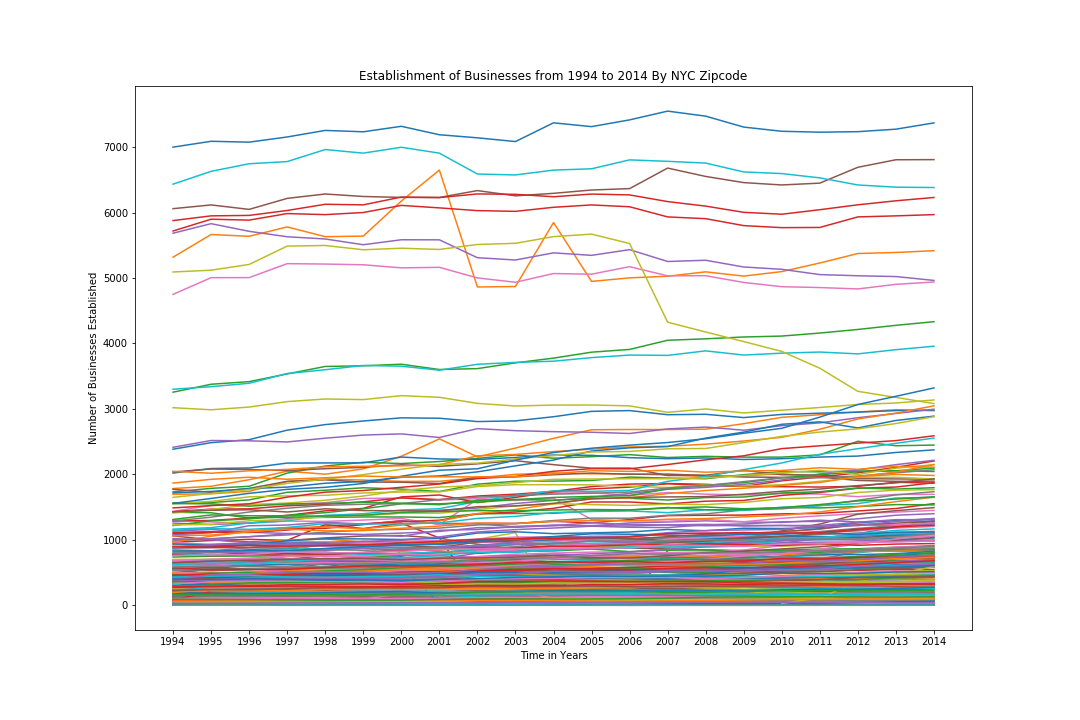
\includegraphics[width=\textwidth]{nonnormalized.png}
		\end{figure}
		
		\noindent As such, to provide a plot that is much more informative, we normalized the data by averaging the yearly value for all Zip Codes and using that average to determine how many standard deviations a Zip Code is from the city, annual average. For a static view of just one year, you can see a distribution of growth and decline. When you add a dynamic view of a time series, you begin to see a greater pattern emerge.
		
		\begin{figure}[H]
			\centering
			\caption{Time Series of Each NYC Zip Code Yearly Mean Normalized}
			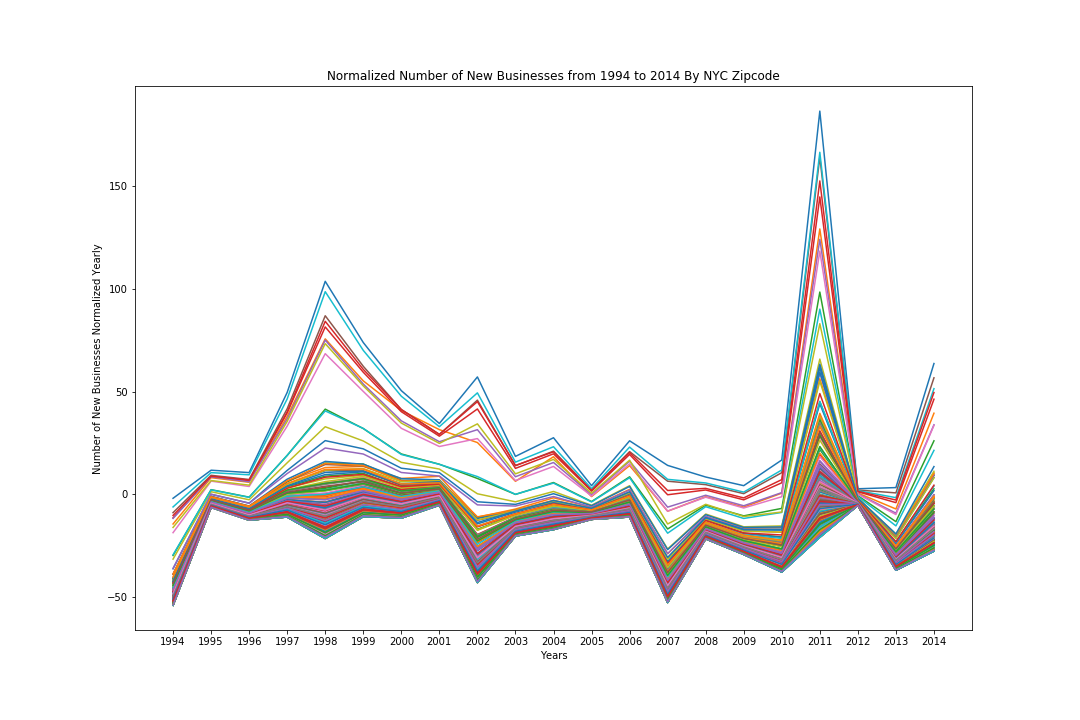
\includegraphics[width=\textwidth]{normalized.png}
			\begin{lstlisting}[language=python]
				arrayData = yearsData.as_matrix()
				arrayData[isnan(arrayData)] = 0
				
				means = np.mean(arrayData, axis=1)
				stds = np.std(arrayData, axis=1)
				
				for index, value in np.ndenumerate(arrayData):
					arrayData[index] = (value - means[index[1]]) / stds[index[1]]
				
				flippedData = np.swapaxes(arrayData, 1, 0)
				flippedData.shape
				
				plt.figure(figsize=(15,10))
				plt.plot(flippedData);
				plt.title("Normalized Number of New Businesses from 1994 to 2014 By NYC Zipcode")
				plt.xlabel("Years")
				xticks(np.arange(0, 21, step=1), np.arange(1994, 2015, step=1))
				plt.ylabel("Number of New Businesses Normalized Yearly")
				plt.savefig('normalized.png');
			\end{lstlisting}
		\end{figure}	
		
		\noindent We begin to see a change in deviation from the mean for each Zip Code over time. Moreover, we begin to see potential clusters of patterns of temporal change. Some changes mirror each other in opposite values while others follow one another. For instance, around 2002, we see a great divergence with some areas increasing business growth while others decline. Perhaps this is due to an event like the 9/11 attacks, with Lower Manhattan closing and losing businesses, while other parts of the city then begin to grow to make up for that loss. Around the Great Recession, we see that some areas are more affected than other areas, though they all follow the same trend. This demonstrates differences in intensity. Thus, with this, we can begin to try to cluster patterns of temporal change.

		\pagebreak
	
	
	\subsection{Elbow Method}
	
		Before we begin using clustering methods, we should determine the number of clusters we should use. A common method, especially for K Means clustering, is the "elbow method". By plotting number of clusters against the sum of squared errors, we see a trade off between SSE and number of clusters. We want as few as possible for both. Thus finding the point where distortion change begin to level, we can say we have found the optimal number of clusters. The elbow method is subject to some degree of subjectivity. One must estimate at what point do we begin to see a lessening of explanatory power. Here, the change between 3 to 4 and 4 to 5 so that 4 is the greatest number of clusters necessary. One could possibly argue for 3 clusters. 
		
		\begin{figure}[H]
			\centering
			\caption{Plot of Optimal Number of Clusters}
			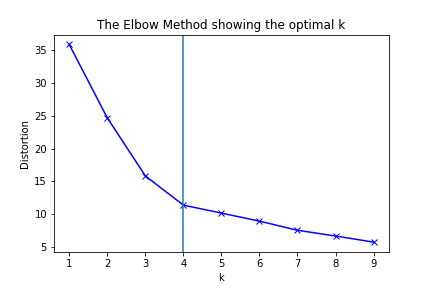
\includegraphics[width=\textwidth]{elbow.png}
		\end{figure}
		
		\begin{figure}[H]
			\centering
			\begin{lstlisting}[language=python]
				distortions = []
				K = range(1,10)
				for k in K:
				kmeanModel = sklearn.cluster.KMeans(n_clusters=k).fit(arrayData)
				kmeanModel.fit(arrayData)
				distortions.append(sum(np.min(cdist(arrayData, kmeanModel.cluster_centers_, 'euclidean'), axis=1)) / arrayData.shape[0])
				
				plt.plot(K, distortions, 'bx-')
				plt.xlabel('k')
				plt.ylabel('Distortion')
				plt.title('The Elbow Method showing the optimal k')
				plt.axvline(x=4)
				plt.savefig("elbow.png")
				plt.show()
			\end{lstlisting}
		\end{figure}	

		\pagebreak

	
	\subsection{K Means Clustering}
	
		The first method we use is K Means clustering, an unsupervised method that works by first randomly assigning k number of centroids where k is the number of clusters as we have determined before. It then iterates many times assigning each data point to the nearest centroid, attempting to minimize distance. After each time of this, centroids are recomputed by taking the mean of all data points assigned to that centroid cluster and starting the process of assignment by minimization again. The below code uses the Python scikit.learn library to use KMeans. First you create a model and then you fit the data to that model.
		
		\begin{figure}[H]
			\centering
			\begin{lstlisting}[language=python]
				k = 4
				kmeanModel = sklearn.cluster.KMeans(n_clusters=k).fit(arrayData)
				kmeanModel.fit(arrayData)
				labels = kmeanModel.fit_predict(arrayData)
				yearsData['clusters'] = kmeanModel.labels_
			\end{lstlisting}			
		\end{figure}
		
		\pagebreak
	
		\noindent Here we have graphed the values of observations by each cluster it has been assigned. The black line represents the center of the cluster, e.g. the mean. 
	
		\begin{figure}[H]
			\centering
			\vspace{5pt}
			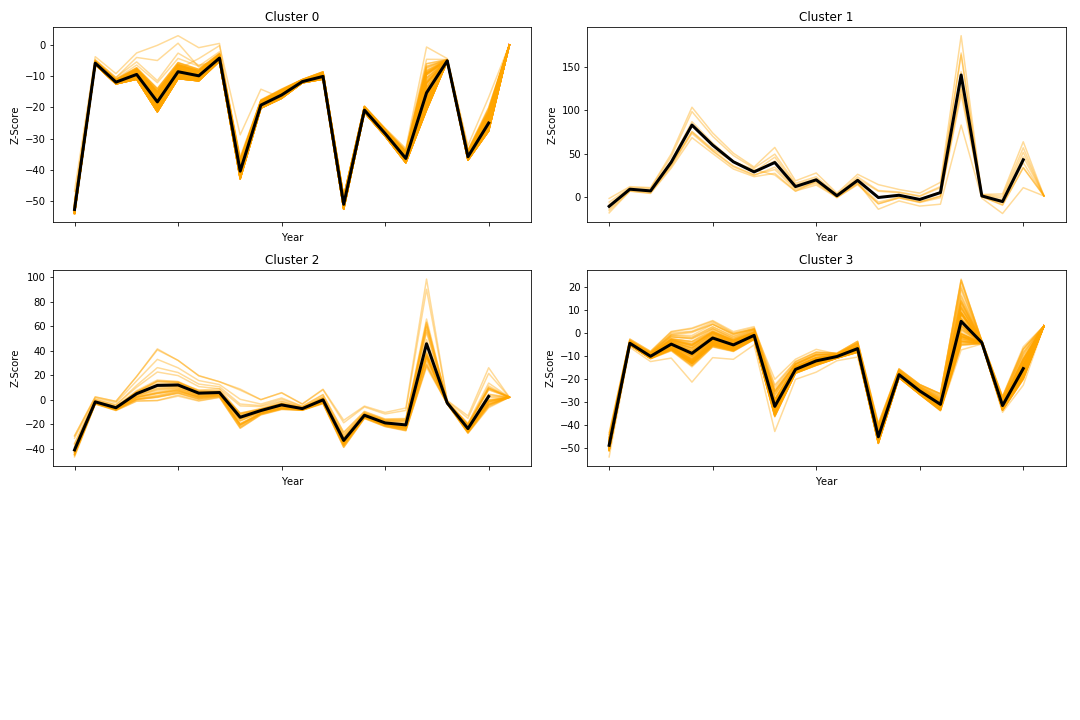
\includegraphics[scale=.25]{clusters.png}
		\end{figure}
		
		\noindent To make it clearer, here we have graphed each mean or cluster center in the same plot to see differences in patterns.
		
		\begin{figure}[H]
			\centering
			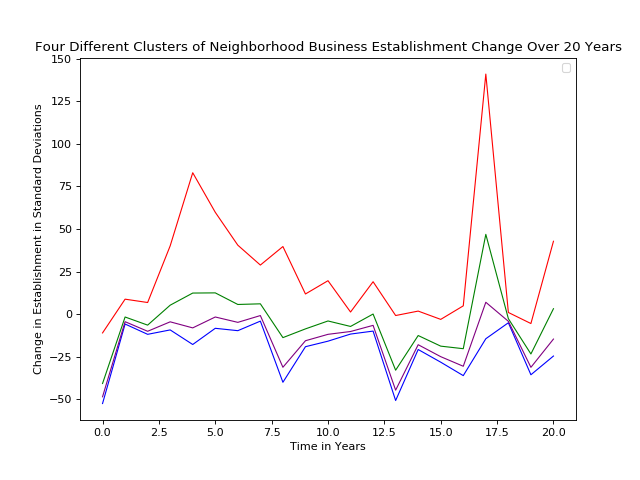
\includegraphics[scale=.5]{means1.png}
		\end{figure}
		
		\pagebreak
	

	
	\subsection{Agglomerative Clustering}
	
		Here, we will try another clustering method. Agglomerative clustering is a form of hierarchical clustering. Rather than be divisive - or "top down" - agglomerative is "bottom up" starting with each observation as its own cluster and then pairing clusters iteratively up until you have the predetermined number of clusters. Again, in the code below, we use the scikit.learn library.

		\begin{figure}[H]
			\centering
			\begin{lstlisting}[language=python]
				k = 4
				agglomModel = sklearn.cluster.AgglomerativeClustering(n_clusters=k).fit(arrayData)
				agglomModel.fit(arrayData)
				labels1 = agglomModel.fit_predict(arrayData)
				yearsData1 = yearsData
				yearsData1['clusters'] = agglomModel.labels_
			\end{lstlisting}			
		\end{figure}
		
		\noindent As before, we plot all the observations in orange separating them into plots by their cluster. The black lines then represent the centers of the clusters or the mean. To make comparison easier, we then plot all the cluster centers together.

		\begin{figure}[H]
			\centering
			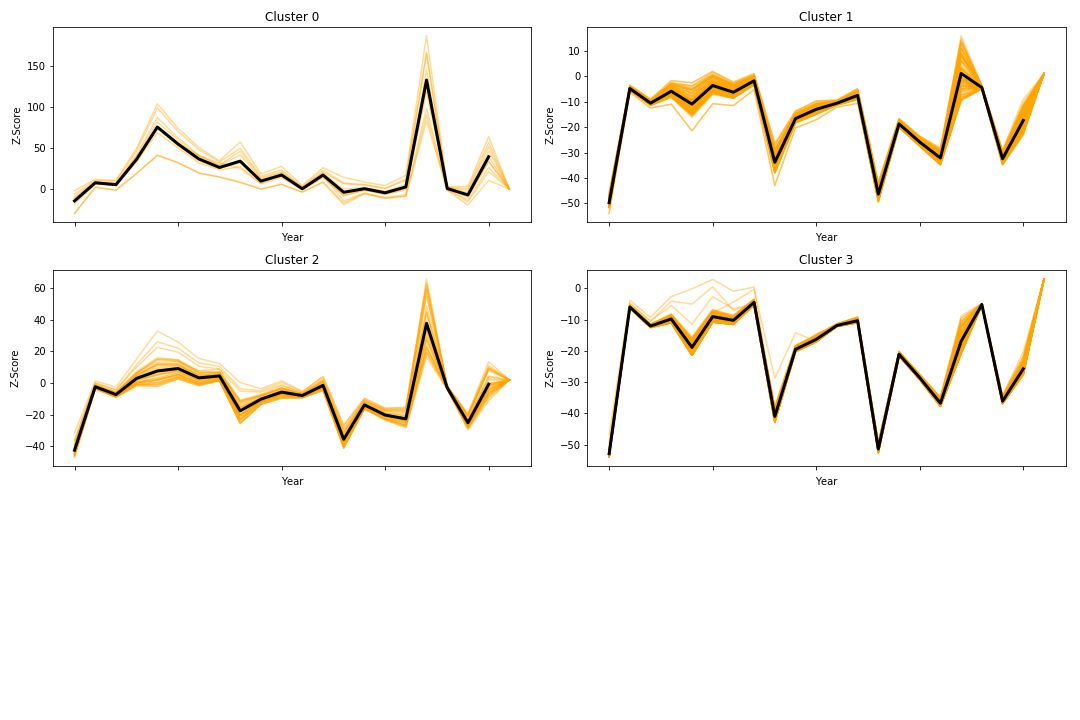
\includegraphics[scale=.25]{clusters1.png}
			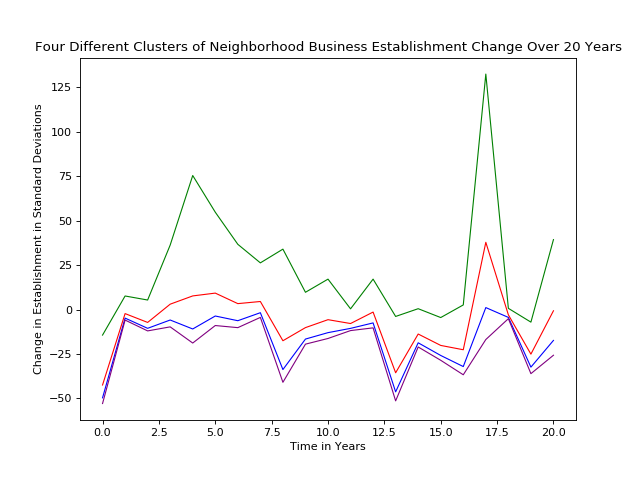
\includegraphics[scale=.5]{means2.png}
		\end{figure}	
		
		\pagebreak
	
	\subsection{Comparing Methods}
	
		If we plot the difference of each different method's cluster means, then we should see how wide the difference is between the two clustering methods. As we see in the below figure, the difference is quite negligible, meaning either method produces similar outcomes.
	
		\begin{figure}[H]
			\centering
			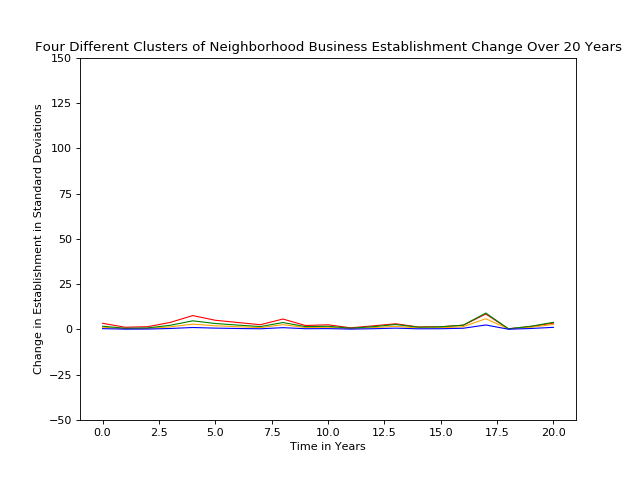
\includegraphics[width=\textwidth]{difference.png}
		\end{figure}	

		\pagebreak
		



\section{Interpretation \& Policy Ramifications}

	\subsection{Interpreting the Clusters Temporally}
	
		We have four different clusters each with somewhat unique temporal patterns of economic growth and decline. Using the K Means clustering, we see that Cluster 0 stays below the mean with volatility. Cluster 3 is quite similar, however is it slightly above Cluster 0. Cluster 2 flits around the mean, beginning slightly above and dipping in 2001 but making a recovery a few years later only to crash again. So far Clusters 0 and 3 are quite volatile with business creation below the city mean. Declines can even be interpreted as loss of businesses, though it could also be interpreted as falling behind as other parts of the city do better. Cluster 2 tries to stay near the city average with bouts above and below average. Finally, it is Cluster 1 that is almost always above the mean. In the Dot Com Boom era, you can see tremendous growth followed by the Dot Com Bust. However, growth is still above the mean, even if it is quite lower. Then one can see the "irrational exuberance" before the Great Recession followed by its market correction. What these clusters are telling us is there are really three economic stories for New York neighborhoods. Some have done tremendously well, rising with booms and even though they fall with busts they still stay above the water. There are neighborhoods that stay around average, sometimes their heads above water and sometimes below. Finally, there are neighborhoods that constantly perform below average with quite some volatility. 
		
	\subsection{Divergent \& Convergent Trends}
	
		These stories become more interesting when compared to one another. Cluster 1 is quite "peaky", with declines during the Dot Com Bust staggered with moments of upturn. Other neighborhoods, however, during the Dot Com Boom, plateau. Interestingly, these neighborhoods decline sharply around the 9/11 attacks while Cluster 1 neighborhoods have a momentary uptick. Over the next few years, the neighborhood begins to converge. Right before the Great Recession, the difference in magnitude between Cluster 1 and other neighborhoods is tremendous. The tides did raise all boats, but some boats were raised much higher than others. Finally, the slope of recovery is different, with Cluster 1 again outperforming others. 
	
	\subsection{Interpreting the Clusters Spatially}
	
		To understand things spatially, we created a choropleth of all the Zip Codes of New York City coded by their Cluster. We find something quite interesting and perhaps against what we would have expected. Midtown Manhattan has seemed to have quite a great deal of disturbance and loss economically. In combination, far out reaches of outer boroughs have seen similar patterns, though this is more in line with expectations. Finally, the areas with high growth include some areas that have become quite popular, such as Downtown Brooklyn and Long Island City. Growth may be indicative of gentrification while shrinkage could be indicative of economic hardship. For instance, Midtown's economic hardship could be more evidence and argument for the planned upzoning to lure more businesses back in the area.
		
		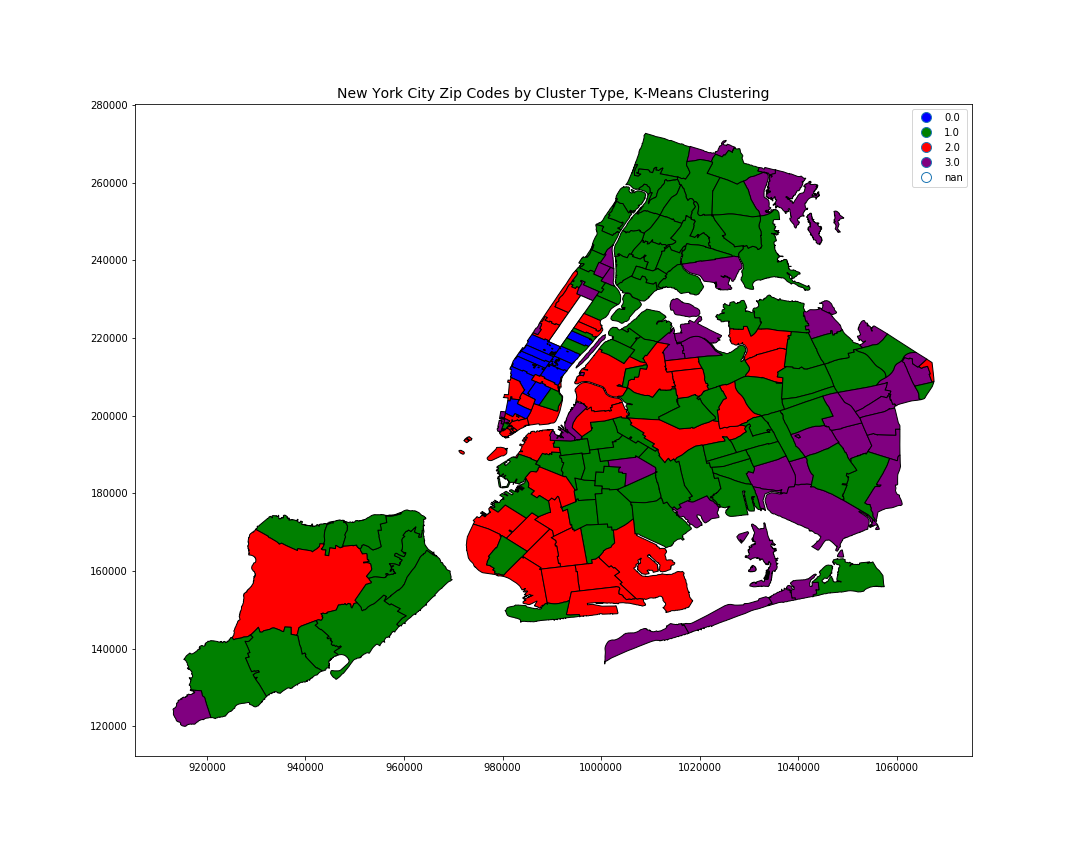
\includegraphics[width=\textwidth]{map.png}

	\pagebreak


\section{Conclusion}
Economic growth is not spatially equal. Certain areas grow more than others and some areas even decline. If we lay out these spatial and temporal distributions against other spatial and temporal patterns, we can begin to see links that help inform good policymaking. Perhaps we see chronically underperforming areas or we see differences in magnitude in change. In the future, we would like to compare different time series and mark individual events as well as compare the distribution spatially with other spatial distributions.



%----------------------------------------------------------------------------------------

\end{document}